\documentclass[12pt,twocolumn]{extarticle}

\PassOptionsToPackage{hyphens}{url}
\usepackage[margin=0.7in]{geometry}
\usepackage{cite}
\usepackage{graphicx}
\usepackage[hyphens]{url}
\usepackage{xurl}
\usepackage{booktabs}
\usepackage{amsmath}
\usepackage{times}
\usepackage[hidelinks]{hyperref}

\setlength{\emergencystretch}{3em}
\Urlmuskip=0mu plus 2mu\relax

\newcommand{\namedurl}[2]{\href{#2}{#1}}

\title{Multi-Language Audio Retrieval for Code-Switched DRC Speech}

\author{Athanase Bahizire \& Stephen N'nouka A. Issah\\
Carnegie Mellon University\\
Applications of AI in Africa, Spring 2026\\
abahizir@andrew.cmu.edu, nnnoukaa@andrew.cmu.edu}

\date{}

\begin{document}

\maketitle

\begin{abstract}
We address a practical data gap for multilingual speech technology in the eastern Democratic Republic of Congo: the lack of usable French--Swahili--Lingala code-switched resources for retrieval experiments. This project produced three outputs: a released synthetic trilingual corpus, a baseline retrieval benchmark over the synthesized text, and a community data-collection web application to support future real speech acquisition. The released corpus contains 9{,}000 text records and 623 aligned synthetic audio clips with frozen train, development, and test splits. On a controlled 164-query benchmark with 50 candidates per query, a TF-IDF word-bigram baseline achieves 0.5803 mean reciprocal rank, 0.4085 Recall@1, and 0.6232 nDCG@5. These results show that the benchmark pipeline works end to end, but they should be interpreted as evidence about this synthetic corpus rather than spontaneous DRC speech.
\end{abstract}

\section{Introduction}
Multilingual speech systems for the DRC face a basic resource problem: there is no ready-to-use French--Swahili--Lingala code-switched corpus for retrieval or speech modeling. Existing multilingual encoders are useful only if appropriate data exists. Our first milestone therefore focused on building data, then using that data to define a reproducible benchmark.

This phase delivered three concrete artifacts. First, we synthesized a trilingual code-switched corpus and released it at \namedurl{the Hugging Face dataset page}{https://huggingface.co/datasets/nnoukastephen/CodeSwitch-SW-LIN-FRA-synthetic-audio}~\cite{hf-dataset}. Second, we scaffolded a community collection web application in \namedurl{the Lilics repository}{https://github.com/Nnouka/CodeSwitch-SW-LIN-FRA-synthetic-audio/tree/master/lilics}~\cite{lilics-repo} for future real-data acquisition. Third, we implemented a baseline experimentation pipeline, documented in \namedurl{the experimentation notebook}{https://github.com/Nnouka/CodeSwitch-SW-LIN-FRA-synthetic-audio/blob/master/experimentation.ipynb}~\cite{experimentation-notebook}, that exports benchmark artifacts and summary analyses to the \texttt{experiment\_outputs} directory.

The central question was intentionally modest: can we create a reproducible synthetic dataset and verify that a simple retrieval baseline operates correctly on it? The answer is yes, with an important limitation. All claims in this report apply to the released synthetic corpus, not to natural conversational speech in general.

\section{Methodology}
\subsection{Datasets and Motivation}
The primary experimental resource is the synthesized text corpus released as \texttt{cs\_text\_dataset.jsonl} under \texttt{synthesis\_outputs/text}. It contains 9{,}000 examples split into 7{,}200 train, 900 development, and 900 test items. Each record stores token-level language tags, matrix language annotations, switch points, and synthesis-quality metadata. This dataset is central because it explicitly models French--Swahili--Lingala code-switching, which was unavailable in existing public resources.

The aligned synthetic audio release contains 623 clips with 498 train, 62 development, and 63 test items. Source material came from parallel French--Lingala and French--Swahili sentence sets downloaded from \namedurl{the Gamayun community site}{https://gamayun.translatorswb.org/data/}~\cite{gamayun-data,gamayun-kit} after we found that the Hugging Face release did not expose aligned pairs in the required format. We also reviewed Common Voice French and WaxalNLP as supporting resources~\cite{common-voice-fr,google-waxalnlp}, but they were not sufficient on their own to define the target trilingual benchmark.

In parallel, we prepared a real-data collection path. The Lilics frontend already supports consent, prompt presentation, recording, metadata submission, and review. This matters because synthetic data is useful for controlled development, but real community data is required for external validity.

\subsection{Text and Audio Synthesis}
The text pipeline normalizes seed examples, applies rule-constrained substitutions inspired by the Matrix Language Frame idea~\cite{myers-scotton1993}, then uses copy-switch bootstrapping to add lexical variation. Swahili is typically retained as the dominant matrix language while French and Lingala spans are inserted at controlled positions. Outputs are filtered by code-switch acceptability and consistency checks before release.

One example is: \emph{Leo tuko na probleme ya maji, mairie ilisema travaux zinaanza kesho matin.} The grammatical frame is mostly Swahili, while French content words are embedded. Similar examples with Lingala spans appear throughout the dataset.

The audio strategy combines synthetic rendering with a future real-speech collection track. We also explored Lingala podcast acquisition, but those recordings were not incorporated because licensing, segmentation, and provenance controls were unresolved.

\subsection{Benchmark Design and Metrics}
The experimentation notebook first defines a text-to-text retrieval benchmark before attempting audio-text retrieval. Using synthesis lineage identifiers, we retained only test items with valid paired targets from the same source family. This yields 164 benchmark queries rather than all 900 test examples. Each query is evaluated against a fixed 50-item candidate set containing one gold target, nine hard negatives, and forty random negatives.

We report mean reciprocal rank (MRR), Recall@1, and nDCG@5. We also compute a code-switch robustness score (CSRS):
\begin{equation}
\mathrm{CSRS} = \frac{\mathrm{MRR}_{\mathrm{high\mbox{-}switch}}}{\mathrm{MRR}_{\mathrm{low\mbox{-}switch}}}.
\end{equation}
The pipeline additionally implements paired bootstrap testing for ranking metrics and McNemar's test for Recall@1, but this milestone executed only a single baseline model, so the significance framework was validated only through a self-comparison sanity check.

\section{Results}
\subsection{Released Resources}
The main deliverable is a released trilingual synthetic corpus with text, audio manifests, and frozen data splits. Table~\ref{tab:summary} summarizes the dataset and baseline benchmark.

\begin{table}[t]
\centering
\caption{Corpus and baseline benchmark summary.}
\label{tab:summary}
\begin{tabular}{@{}lr@{}}
\toprule
Item & Value \\
\midrule
Text records & 9{,}000 \\
Text split & 7{,}200 / 900 / 900 \\
Audio clips & 623 \\
Audio split & 498 / 62 / 63 \\
Benchmark queries & 164 \\
Candidates per query & 50 \\
MRR & 0.5803 \\
Recall@1 & 0.4085 \\
nDCG@5 & 0.6232 \\
CSRS & 1.4277 \\
\bottomrule
\end{tabular}
\end{table}

\subsection{Baseline Retrieval Performance}
We executed a TF-IDF word-bigram baseline. The purpose of this model is not to set a strong state of the art; it verifies that the candidate-pool construction, ranking, metric computation, and export pipeline work correctly end to end.

The baseline retrieves the correct sibling example relatively early in many rankings, which is expected because positive pairs come from related synthetic lineages and therefore retain lexical overlap. This is useful as a debugging baseline, but it also means the scores should not be interpreted as evidence that the same method would generalize to natural speech.

\begin{figure}[t]
\centering
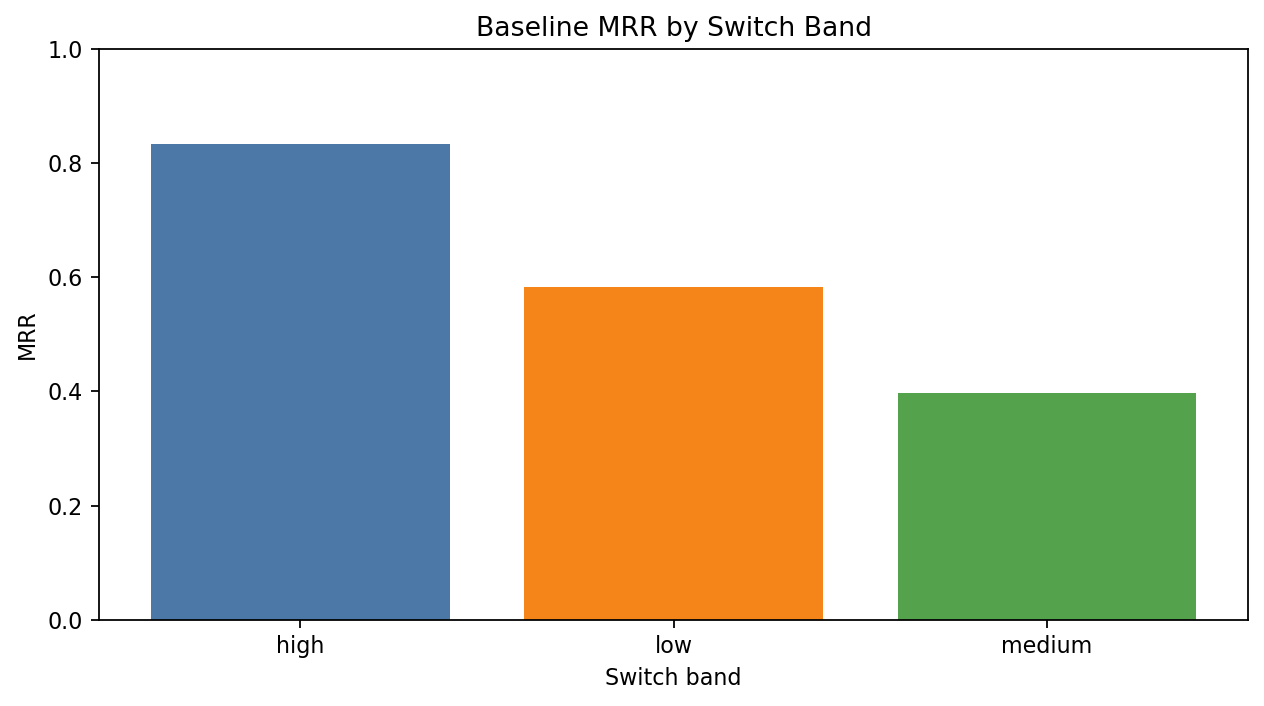
\includegraphics[width=\columnwidth]{experiment_outputs/plots/baseline_mrr_by_switch_band.png}
\caption{Performance varies by switch band; the high-switch subset appears easier but is also small.}
\label{fig:switchband}
\end{figure}

By switch band, the model achieves MRR values of 0.8333 for high-switch examples, 0.5837 for low-switch examples, and 0.3976 for medium-switch examples. The best score on the high-switch subset is counterintuitive and should not be overinterpreted. That subset is small, and its examples appear easier than average. The medium-switch condition is the more plausible failure region in this benchmark.

\begin{figure}[t]
\centering
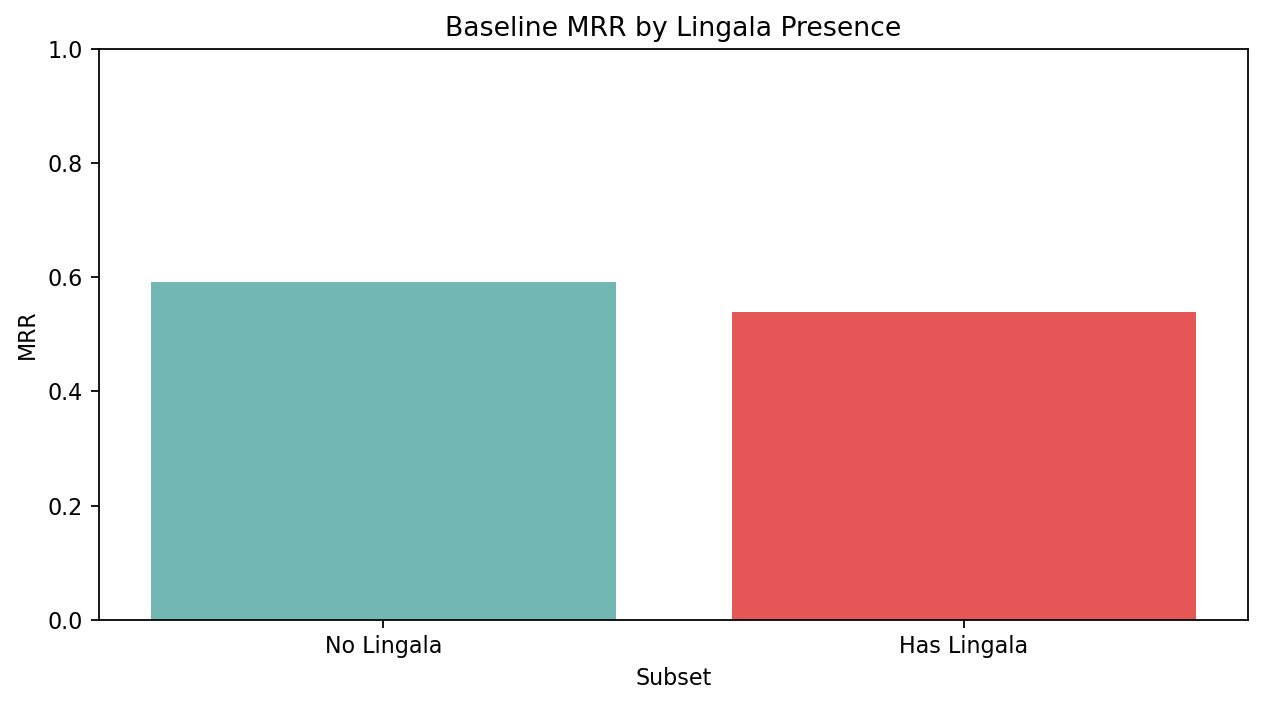
\includegraphics[width=\columnwidth]{experiment_outputs/plots/baseline_mrr_by_lingala_presence.png}
\caption{Lingala-bearing examples show a modest drop in lexical retrieval quality.}
\label{fig:lingala}
\end{figure}

Conditioning on Lingala presence shows a modest degradation: MRR drops from 0.5912 on examples without Lingala to 0.5385 when Lingala is present. Recall@1 and nDCG@5 follow the same trend. This is consistent with the smaller amount of Lingala-bearing material and with the weaker lexical regularity available to a simple bag-of-ngrams baseline.

\subsection{Error Analysis}
A common failure mode is lexical-topic confusion. The model often retrieves a sentence with many overlapping topical words but misses the intended paired target because several generated examples are near-duplicates that differ in only a few tokens. This is informative rather than incidental: the errors show that the benchmark negatives are genuinely hard and that the current setup can distinguish partial lexical overlap from exact paired retrieval.

\section{Discussion}
This milestone's main contribution is experimental infrastructure rather than a strong model. We now have a released trilingual synthetic corpus, a reproducible retrieval benchmark, exported result summaries, and an initial real-data collection application. Those pieces remove the project's main early blocker: the absence of usable data.

Two conclusions are justified. First, the synthetic corpus is rich enough to support controlled retrieval experiments. Second, the present benchmark remains dominated by synthetic similarity structure, especially lexical overlap among paired siblings. The current numbers are therefore best viewed as a baseline for future comparison, not as a claim about real-world conversational retrieval in the DRC.

The significance-testing code is in place, but this report does not present a meaningful significance comparison because only one actual baseline model was run. The next scientifically useful step is to compare stronger multilingual encoders or audio-text models against the same frozen benchmark and apply the existing statistical tests to those comparisons. Candidate next baselines include SERENGETI~\cite{serengeti}, AfriBERTa~\cite{afriberta}, and multilingual audio-text backbones built from WaxalNLP supervision~\cite{google-waxalnlp}.

\section{Conclusion}
We converted an open-ended project idea into a concrete experimental asset: a released French--Swahili--Lingala synthetic corpus with 9{,}000 text records and 623 aligned audio clips, plus a controlled 164-query retrieval benchmark. A simple TF-IDF baseline reaches 0.5803 MRR, 0.4085 Recall@1, and 0.6232 nDCG@5, confirming that the pipeline operates correctly. The main limitation is external validity: the benchmark is still synthetic. The practical value of this phase is that it establishes the data, tooling, and collection workflow needed for stronger multilingual retrieval experiments on future community-sourced speech.

\bibliographystyle{plain}
\bibliography{reference}

\end{document}
